\documentclass[]{article}
\usepackage{lmodern}
\usepackage{amssymb,amsmath}
\usepackage{ifxetex,ifluatex}
\usepackage{fixltx2e} % provides \textsubscript
\ifnum 0\ifxetex 1\fi\ifluatex 1\fi=0 % if pdftex
  \usepackage[T1]{fontenc}
  \usepackage[utf8]{inputenc}
\else % if luatex or xelatex
  \ifxetex
    \usepackage{mathspec}
  \else
    \usepackage{fontspec}
  \fi
  \defaultfontfeatures{Ligatures=TeX,Scale=MatchLowercase}
\fi
% use upquote if available, for straight quotes in verbatim environments
\IfFileExists{upquote.sty}{\usepackage{upquote}}{}
% use microtype if available
\IfFileExists{microtype.sty}{%
\usepackage{microtype}
\UseMicrotypeSet[protrusion]{basicmath} % disable protrusion for tt fonts
}{}
\usepackage[margin=2.54cm]{geometry}
\usepackage{hyperref}
\hypersetup{unicode=true,
            pdftitle={Assignment 8: Time Series Analysis},
            pdfauthor={Siying Chen},
            pdfborder={0 0 0},
            breaklinks=true}
\urlstyle{same}  % don't use monospace font for urls
\usepackage{color}
\usepackage{fancyvrb}
\newcommand{\VerbBar}{|}
\newcommand{\VERB}{\Verb[commandchars=\\\{\}]}
\DefineVerbatimEnvironment{Highlighting}{Verbatim}{commandchars=\\\{\}}
% Add ',fontsize=\small' for more characters per line
\usepackage{framed}
\definecolor{shadecolor}{RGB}{248,248,248}
\newenvironment{Shaded}{\begin{snugshade}}{\end{snugshade}}
\newcommand{\KeywordTok}[1]{\textcolor[rgb]{0.13,0.29,0.53}{\textbf{#1}}}
\newcommand{\DataTypeTok}[1]{\textcolor[rgb]{0.13,0.29,0.53}{#1}}
\newcommand{\DecValTok}[1]{\textcolor[rgb]{0.00,0.00,0.81}{#1}}
\newcommand{\BaseNTok}[1]{\textcolor[rgb]{0.00,0.00,0.81}{#1}}
\newcommand{\FloatTok}[1]{\textcolor[rgb]{0.00,0.00,0.81}{#1}}
\newcommand{\ConstantTok}[1]{\textcolor[rgb]{0.00,0.00,0.00}{#1}}
\newcommand{\CharTok}[1]{\textcolor[rgb]{0.31,0.60,0.02}{#1}}
\newcommand{\SpecialCharTok}[1]{\textcolor[rgb]{0.00,0.00,0.00}{#1}}
\newcommand{\StringTok}[1]{\textcolor[rgb]{0.31,0.60,0.02}{#1}}
\newcommand{\VerbatimStringTok}[1]{\textcolor[rgb]{0.31,0.60,0.02}{#1}}
\newcommand{\SpecialStringTok}[1]{\textcolor[rgb]{0.31,0.60,0.02}{#1}}
\newcommand{\ImportTok}[1]{#1}
\newcommand{\CommentTok}[1]{\textcolor[rgb]{0.56,0.35,0.01}{\textit{#1}}}
\newcommand{\DocumentationTok}[1]{\textcolor[rgb]{0.56,0.35,0.01}{\textbf{\textit{#1}}}}
\newcommand{\AnnotationTok}[1]{\textcolor[rgb]{0.56,0.35,0.01}{\textbf{\textit{#1}}}}
\newcommand{\CommentVarTok}[1]{\textcolor[rgb]{0.56,0.35,0.01}{\textbf{\textit{#1}}}}
\newcommand{\OtherTok}[1]{\textcolor[rgb]{0.56,0.35,0.01}{#1}}
\newcommand{\FunctionTok}[1]{\textcolor[rgb]{0.00,0.00,0.00}{#1}}
\newcommand{\VariableTok}[1]{\textcolor[rgb]{0.00,0.00,0.00}{#1}}
\newcommand{\ControlFlowTok}[1]{\textcolor[rgb]{0.13,0.29,0.53}{\textbf{#1}}}
\newcommand{\OperatorTok}[1]{\textcolor[rgb]{0.81,0.36,0.00}{\textbf{#1}}}
\newcommand{\BuiltInTok}[1]{#1}
\newcommand{\ExtensionTok}[1]{#1}
\newcommand{\PreprocessorTok}[1]{\textcolor[rgb]{0.56,0.35,0.01}{\textit{#1}}}
\newcommand{\AttributeTok}[1]{\textcolor[rgb]{0.77,0.63,0.00}{#1}}
\newcommand{\RegionMarkerTok}[1]{#1}
\newcommand{\InformationTok}[1]{\textcolor[rgb]{0.56,0.35,0.01}{\textbf{\textit{#1}}}}
\newcommand{\WarningTok}[1]{\textcolor[rgb]{0.56,0.35,0.01}{\textbf{\textit{#1}}}}
\newcommand{\AlertTok}[1]{\textcolor[rgb]{0.94,0.16,0.16}{#1}}
\newcommand{\ErrorTok}[1]{\textcolor[rgb]{0.64,0.00,0.00}{\textbf{#1}}}
\newcommand{\NormalTok}[1]{#1}
\usepackage{graphicx,grffile}
\makeatletter
\def\maxwidth{\ifdim\Gin@nat@width>\linewidth\linewidth\else\Gin@nat@width\fi}
\def\maxheight{\ifdim\Gin@nat@height>\textheight\textheight\else\Gin@nat@height\fi}
\makeatother
% Scale images if necessary, so that they will not overflow the page
% margins by default, and it is still possible to overwrite the defaults
% using explicit options in \includegraphics[width, height, ...]{}
\setkeys{Gin}{width=\maxwidth,height=\maxheight,keepaspectratio}
\IfFileExists{parskip.sty}{%
\usepackage{parskip}
}{% else
\setlength{\parindent}{0pt}
\setlength{\parskip}{6pt plus 2pt minus 1pt}
}
\setlength{\emergencystretch}{3em}  % prevent overfull lines
\providecommand{\tightlist}{%
  \setlength{\itemsep}{0pt}\setlength{\parskip}{0pt}}
\setcounter{secnumdepth}{0}
% Redefines (sub)paragraphs to behave more like sections
\ifx\paragraph\undefined\else
\let\oldparagraph\paragraph
\renewcommand{\paragraph}[1]{\oldparagraph{#1}\mbox{}}
\fi
\ifx\subparagraph\undefined\else
\let\oldsubparagraph\subparagraph
\renewcommand{\subparagraph}[1]{\oldsubparagraph{#1}\mbox{}}
\fi

%%% Use protect on footnotes to avoid problems with footnotes in titles
\let\rmarkdownfootnote\footnote%
\def\footnote{\protect\rmarkdownfootnote}

%%% Change title format to be more compact
\usepackage{titling}

% Create subtitle command for use in maketitle
\newcommand{\subtitle}[1]{
  \posttitle{
    \begin{center}\large#1\end{center}
    }
}

\setlength{\droptitle}{-2em}

  \title{Assignment 8: Time Series Analysis}
    \pretitle{\vspace{\droptitle}\centering\huge}
  \posttitle{\par}
    \author{Siying Chen}
    \preauthor{\centering\large\emph}
  \postauthor{\par}
    \date{}
    \predate{}\postdate{}
  

\begin{document}
\maketitle

\subsection{OVERVIEW}\label{overview}

This exercise accompanies the lessons in Environmental Data Analytics
(ENV872L) on time series analysis.

\subsection{Directions}\label{directions}

\begin{enumerate}
\def\labelenumi{\arabic{enumi}.}
\tightlist
\item
  Change ``Student Name'' on line 3 (above) with your name.
\item
  Use the lesson as a guide. It contains code that can be modified to
  complete the assignment.
\item
  Work through the steps, \textbf{creating code and output} that fulfill
  each instruction.
\item
  Be sure to \textbf{answer the questions} in this assignment document.
  Space for your answers is provided in this document and is indicated
  by the ``\textgreater{}'' character. If you need a second paragraph be
  sure to start the first line with ``\textgreater{}''. You should
  notice that the answer is highlighted in green by RStudio.
\item
  When you have completed the assignment, \textbf{Knit} the text and
  code into a single PDF file. You will need to have the correct
  software installed to do this (see Software Installation Guide) Press
  the \texttt{Knit} button in the RStudio scripting panel. This will
  save the PDF output in your Assignments folder.
\item
  After Knitting, please submit the completed exercise (PDF file) to the
  dropbox in Sakai. Please add your last name into the file name (e.g.,
  ``Salk\_A08\_TimeSeries.pdf'') prior to submission.
\end{enumerate}

The completed exercise is due on Tuesday, 19 March, 2019 before class
begins.

\subsection{Brainstorm a project
topic}\label{brainstorm-a-project-topic}

\begin{enumerate}
\def\labelenumi{\arabic{enumi}.}
\tightlist
\item
  Spend 15 minutes brainstorming ideas for a project topic, and look for
  a dataset if you are choosing your own rather than using a class
  dataset. Remember your topic choices are due by the end of March, and
  you should post your choice ASAP to the forum on Sakai.
\end{enumerate}

Question: Did you do this?

\begin{quote}
ANSWER: Yes. I'll use the NTL\_LTER nutrient and chemical/physical
dataset along with the phytoplankton dataset I found online and perform
time series analysis to find out the relationship between phytoplankton
and nutrients/D.O./irradiance over time.
\end{quote}

\subsection{Set up your session}\label{set-up-your-session}

\begin{enumerate}
\def\labelenumi{\arabic{enumi}.}
\setcounter{enumi}{1}
\tightlist
\item
  Set up your session. Upload the EPA air quality raw dataset for PM2.5
  in 2018, and the processed NTL-LTER dataset for nutrients in Peter and
  Paul lakes. Build a ggplot theme and set it as your default theme.
  Make sure date variables are set to a date format.
\end{enumerate}

\begin{Shaded}
\begin{Highlighting}[]
\KeywordTok{getwd}\NormalTok{()}
\end{Highlighting}
\end{Shaded}

\begin{verbatim}
## [1] "/Users/Sylvia/Downloads/ENV872/ENV872"
\end{verbatim}

\begin{Shaded}
\begin{Highlighting}[]
\KeywordTok{library}\NormalTok{(tidyverse)}
\end{Highlighting}
\end{Shaded}

\begin{verbatim}
## -- Attaching packages -------------------------------------------------------------------- tidyverse 1.2.1 --
\end{verbatim}

\begin{verbatim}
## v ggplot2 3.1.0     v purrr   0.2.5
## v tibble  2.0.1     v dplyr   0.7.8
## v tidyr   0.8.2     v stringr 1.3.1
## v readr   1.3.1     v forcats 0.3.0
\end{verbatim}

\begin{verbatim}
## -- Conflicts ----------------------------------------------------------------------- tidyverse_conflicts() --
## x dplyr::filter() masks stats::filter()
## x dplyr::lag()    masks stats::lag()
\end{verbatim}

\begin{Shaded}
\begin{Highlighting}[]
\KeywordTok{library}\NormalTok{(lubridate)}
\end{Highlighting}
\end{Shaded}

\begin{verbatim}
## 
## Attaching package: 'lubridate'
\end{verbatim}

\begin{verbatim}
## The following object is masked from 'package:base':
## 
##     date
\end{verbatim}

\begin{Shaded}
\begin{Highlighting}[]
\KeywordTok{library}\NormalTok{(nlme)}
\end{Highlighting}
\end{Shaded}

\begin{verbatim}
## 
## Attaching package: 'nlme'
\end{verbatim}

\begin{verbatim}
## The following object is masked from 'package:dplyr':
## 
##     collapse
\end{verbatim}

\begin{Shaded}
\begin{Highlighting}[]
\KeywordTok{library}\NormalTok{(lsmeans)}
\end{Highlighting}
\end{Shaded}

\begin{verbatim}
## Loading required package: emmeans
\end{verbatim}

\begin{verbatim}
## The 'lsmeans' package is now basically a front end for 'emmeans'.
## Users are encouraged to switch the rest of the way.
## See help('transition') for more information, including how to
## convert old 'lsmeans' objects and scripts to work with 'emmeans'.
\end{verbatim}

\begin{Shaded}
\begin{Highlighting}[]
\KeywordTok{library}\NormalTok{(multcompView)}
\KeywordTok{library}\NormalTok{(trend)}

\NormalTok{PM2.}\DecValTok{5}\NormalTok{ <-}\StringTok{ }\KeywordTok{read.csv}\NormalTok{(}\StringTok{"./Data/Raw/EPAair_PM25_NC2018_raw.csv"}\NormalTok{)}
\NormalTok{PM2.}\DecValTok{5}\OperatorTok{$}\NormalTok{Date <-}\StringTok{ }\KeywordTok{as.Date}\NormalTok{(PM2.}\DecValTok{5}\OperatorTok{$}\NormalTok{Date, }\DataTypeTok{format =} \StringTok{"%m/%d/%y"}\NormalTok{)}

\NormalTok{PeterPaul.nutrients <-}\StringTok{ }\KeywordTok{read.csv}\NormalTok{(}\StringTok{"./Data/Processed/NTL-LTER_Lake_Nutrients_PeterPaul_Processed.csv"}\NormalTok{)}
\NormalTok{PeterPaul.nutrients}\OperatorTok{$}\NormalTok{sampledate <-}\StringTok{ }\KeywordTok{as.Date}\NormalTok{(PeterPaul.nutrients}\OperatorTok{$}\NormalTok{sampledate, }\DataTypeTok{format =} \StringTok{"%Y-%m-%d"}\NormalTok{)}

\NormalTok{mytheme <-}\StringTok{ }\KeywordTok{theme_bw}\NormalTok{(}\DataTypeTok{base_size =} \DecValTok{14}\NormalTok{) }\OperatorTok{+}
\StringTok{  }\KeywordTok{theme}\NormalTok{(}\DataTypeTok{axis.text =} \KeywordTok{element_text}\NormalTok{(}\DataTypeTok{color =} \StringTok{"black"}\NormalTok{), }
        \DataTypeTok{legend.position =} \StringTok{"bottom"}\NormalTok{,}
        \DataTypeTok{panel.grid.major =} \KeywordTok{element_line}\NormalTok{(}\DataTypeTok{size =} \FloatTok{0.5}\NormalTok{, }\DataTypeTok{linetype =} \StringTok{'solid'}\NormalTok{), }
        \DataTypeTok{panel.grid.minor =} \KeywordTok{element_line}\NormalTok{(}\DataTypeTok{size =} \FloatTok{0.25}\NormalTok{, }\DataTypeTok{linetype =} \StringTok{'dashed'}\NormalTok{),}
        \DataTypeTok{title =} \KeywordTok{element_text}\NormalTok{(}\DataTypeTok{face =} \StringTok{"bold"}\NormalTok{))}
\KeywordTok{theme_set}\NormalTok{(mytheme)}
\end{Highlighting}
\end{Shaded}

\subsection{Run a hierarchical (mixed-effects)
model}\label{run-a-hierarchical-mixed-effects-model}

Research question: Do PM2.5 concentrations have a significant trend in
2018?

\begin{enumerate}
\def\labelenumi{\arabic{enumi}.}
\setcounter{enumi}{2}
\tightlist
\item
  Run a repeated measures ANOVA, with PM2.5 concentrations as the
  response, Date as a fixed effect, and Site.Name as a random effect.
  This will allow us to extrapolate PM2.5 concentrations across North
  Carolina.
\end{enumerate}

3a. Illustrate PM2.5 concentrations by date. Do not split aesthetics by
site.

\begin{Shaded}
\begin{Highlighting}[]
\NormalTok{PM2.}\FloatTok{5.}\NormalTok{plot <-}\StringTok{ }\KeywordTok{ggplot}\NormalTok{(PM2.}\DecValTok{5}\NormalTok{, }\KeywordTok{aes}\NormalTok{(}\DataTypeTok{x =}\NormalTok{ Date, }\DataTypeTok{y =}\NormalTok{ Daily.Mean.PM2.}\FloatTok{5.}\NormalTok{Concentration)) }\OperatorTok{+}
\StringTok{  }\KeywordTok{geom_point}\NormalTok{(}\DataTypeTok{alpha =} \FloatTok{0.3}\NormalTok{) }\OperatorTok{+}
\StringTok{  }\KeywordTok{ylab}\NormalTok{(}\StringTok{"Daily Mean PM 2.5 Concentration"}\NormalTok{) }\OperatorTok{+}
\StringTok{  }\KeywordTok{scale_x_date}\NormalTok{(}\DataTypeTok{date_breaks =} \StringTok{"1 month"}\NormalTok{) }\OperatorTok{+}
\StringTok{  }\KeywordTok{theme}\NormalTok{(}\DataTypeTok{axis.text.x =} \KeywordTok{element_text}\NormalTok{(}\DataTypeTok{angle=}\DecValTok{90}\NormalTok{))}
\KeywordTok{print}\NormalTok{(PM2.}\FloatTok{5.}\NormalTok{plot)}
\end{Highlighting}
\end{Shaded}

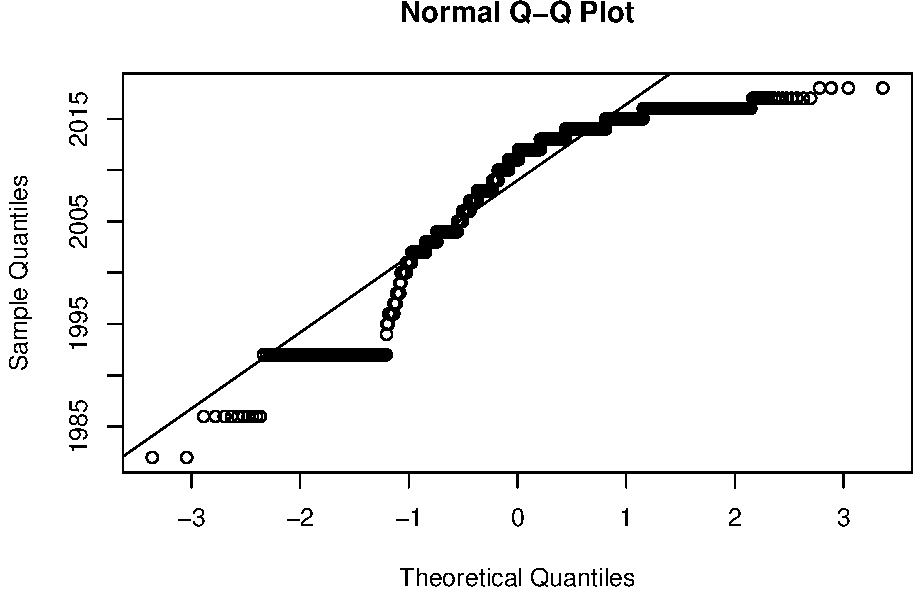
\includegraphics{A08_TimeSeries_files/figure-latex/unnamed-chunk-2-1.pdf}

3b. Insert the following line of code into your R chunk. This will
eliminate duplicate measurements on single dates for each site. PM2.5 =
PM2.5{[}order(PM2.5{[},`Date'{]},-PM2.5{[},`Site.ID'{]}),{]} PM2.5 =
PM2.5{[}!duplicated(PM2.5\$Date),{]}

3c. Determine the temporal autocorrelation in your model.

3d. Run a mixed effects model.

\begin{Shaded}
\begin{Highlighting}[]
\CommentTok{# Remove duplicate data}
\NormalTok{PM2.}\DecValTok{5}\NormalTok{ =}\StringTok{ }\NormalTok{PM2.}\DecValTok{5}\NormalTok{[}\KeywordTok{order}\NormalTok{(PM2.}\DecValTok{5}\NormalTok{[,}\StringTok{'Date'}\NormalTok{],}\OperatorTok{-}\NormalTok{PM2.}\DecValTok{5}\NormalTok{[,}\StringTok{'Site.ID'}\NormalTok{]),]}
\NormalTok{PM2.}\DecValTok{5}\NormalTok{ =}\StringTok{ }\NormalTok{PM2.}\DecValTok{5}\NormalTok{[}\OperatorTok{!}\KeywordTok{duplicated}\NormalTok{(PM2.}\DecValTok{5}\OperatorTok{$}\NormalTok{Date),]}

\CommentTok{# Temporal autocorrelation test}
\NormalTok{PM2.}\FloatTok{5.}\NormalTok{auto <-}\StringTok{ }\KeywordTok{lme}\NormalTok{(}\DataTypeTok{data =}\NormalTok{ PM2.}\DecValTok{5}\NormalTok{,}
\NormalTok{                 Daily.Mean.PM2.}\FloatTok{5.}\NormalTok{Concentration }\OperatorTok{~}\StringTok{ }\NormalTok{Date,}
                 \DataTypeTok{random =} \OperatorTok{~}\DecValTok{1}\OperatorTok{|}\NormalTok{Site.Name)}
\NormalTok{PM2.}\FloatTok{5.}\NormalTok{auto }
\end{Highlighting}
\end{Shaded}

\begin{verbatim}
## Linear mixed-effects model fit by REML
##   Data: PM2.5 
##   Log-restricted-likelihood: -928.6076
##   Fixed: Daily.Mean.PM2.5.Concentration ~ Date 
##  (Intercept)         Date 
## 90.465022634 -0.004727976 
## 
## Random effects:
##  Formula: ~1 | Site.Name
##         (Intercept) Residual
## StdDev:    1.650184 3.559209
## 
## Number of Observations: 343
## Number of Groups: 3
\end{verbatim}

\begin{Shaded}
\begin{Highlighting}[]
\KeywordTok{ACF}\NormalTok{(PM2.}\FloatTok{5.}\NormalTok{auto)}
\end{Highlighting}
\end{Shaded}

\begin{verbatim}
##    lag          ACF
## 1    0  1.000000000
## 2    1  0.513829909
## 3    2  0.194512680
## 4    3  0.117925187
## 5    4  0.126462863
## 6    5  0.100699787
## 7    6  0.058215891
## 8    7 -0.053090104
## 9    8  0.017671857
## 10   9  0.012177847
## 11  10 -0.003699721
## 12  11 -0.020305291
## 13  12 -0.044621086
## 14  13 -0.055602646
## 15  14 -0.065787345
## 16  15 -0.123987593
## 17  16 -0.055414056
## 18  17  0.002911218
## 19  18  0.025133456
## 20  19 -0.015306468
## 21  20 -0.143472007
## 22  21 -0.155495492
## 23  22 -0.060369985
## 24  23  0.003954231
## 25  24  0.042295682
## 26  25  0.001320007
\end{verbatim}

\begin{Shaded}
\begin{Highlighting}[]
\CommentTok{# Mixed effect model}
\NormalTok{PM2.}\FloatTok{5.}\NormalTok{mixed <-}\StringTok{ }\KeywordTok{lme}\NormalTok{(}\DataTypeTok{data =}\NormalTok{ PM2.}\DecValTok{5}\NormalTok{,}
\NormalTok{                  Daily.Mean.PM2.}\FloatTok{5.}\NormalTok{Concentration }\OperatorTok{~}\StringTok{ }\NormalTok{Date, }
                  \DataTypeTok{random =} \OperatorTok{~}\DecValTok{1}\OperatorTok{|}\NormalTok{Site.Name,}
                  \DataTypeTok{correlation =} \KeywordTok{corAR1}\NormalTok{(}\DataTypeTok{form =} \OperatorTok{~}\StringTok{ }\NormalTok{Date}\OperatorTok{|}\NormalTok{Site.Name, }\DataTypeTok{value =} \FloatTok{0.514}\NormalTok{),}
                  \DataTypeTok{method =} \StringTok{"REML"}\NormalTok{)}
\KeywordTok{summary}\NormalTok{(PM2.}\FloatTok{5.}\NormalTok{mixed)}
\end{Highlighting}
\end{Shaded}

\begin{verbatim}
## Linear mixed-effects model fit by REML
##  Data: PM2.5 
##        AIC      BIC   logLik
##   1756.622 1775.781 -873.311
## 
## Random effects:
##  Formula: ~1 | Site.Name
##         (Intercept) Residual
## StdDev: 0.001028133 3.597269
## 
## Correlation Structure: ARMA(1,0)
##  Formula: ~Date | Site.Name 
##  Parameter estimate(s):
##      Phi1 
## 0.5384349 
## Fixed effects: Daily.Mean.PM2.5.Concentration ~ Date 
##                Value Std.Error  DF   t-value p-value
## (Intercept) 83.14801  60.63585 339  1.371268  0.1712
## Date        -0.00426   0.00342 339 -1.244145  0.2143
##  Correlation: 
##      (Intr)
## Date -1    
## 
## Standardized Within-Group Residuals:
##        Min         Q1        Med         Q3        Max 
## -2.3220745 -0.6187194 -0.1116751  0.6164257  3.4192603 
## 
## Number of Observations: 343
## Number of Groups: 3
\end{verbatim}

Is there a significant increasing or decreasing trend in PM2.5
concentrations in 2018?

\begin{quote}
ANSWER: There is no significant trend detected in PM2.5 concentrations
in 2018 since p-value is greater than 0.05.
\end{quote}

3e. Run a fixed effects model with Date as the only explanatory
variable. Then test whether the mixed effects model is a better fit than
the fixed effect model.

\begin{Shaded}
\begin{Highlighting}[]
\NormalTok{PM2.}\FloatTok{5.}\NormalTok{fixed <-}\StringTok{ }\KeywordTok{gls}\NormalTok{(}\DataTypeTok{data =}\NormalTok{ PM2.}\DecValTok{5}\NormalTok{,}
\NormalTok{                   Daily.Mean.PM2.}\FloatTok{5.}\NormalTok{Concentration }\OperatorTok{~}\StringTok{ }\NormalTok{Date }\OperatorTok{*}\StringTok{ }\NormalTok{Site.Name,}
                   \DataTypeTok{method =} \StringTok{"REML"}\NormalTok{)}
\KeywordTok{summary}\NormalTok{(PM2.}\FloatTok{5.}\NormalTok{fixed)}
\end{Highlighting}
\end{Shaded}

\begin{verbatim}
## Generalized least squares fit by REML
##   Model: Daily.Mean.PM2.5.Concentration ~ Date * Site.Name 
##   Data: PM2.5 
##        AIC      BIC    logLik
##   1865.812 1892.552 -925.9059
## 
## Coefficients:
##                                     Value Std.Error    t-value p-value
## (Intercept)                     11540.630 15142.989  0.7621104  0.4465
## Date                               -0.649     0.851 -0.7618782  0.4467
## Site.NameMillbrook School      -11622.193 15144.205 -0.7674350  0.4434
## Site.NameTriple Oak            -11446.924 15143.029 -0.7559203  0.4502
## Date:Site.NameMillbrook School      0.654     0.851  0.7677302  0.4432
## Date:Site.NameTriple Oak            0.644     0.851  0.7561773  0.4501
## 
##  Correlation: 
##                                (Intr) Date St.NMS St.NTO D:S.NS
## Date                           -1                              
## Site.NameMillbrook School      -1      1                       
## Site.NameTriple Oak            -1      1    1                  
## Date:Site.NameMillbrook School  1     -1   -1     -1           
## Date:Site.NameTriple Oak        1     -1   -1     -1      1    
## 
## Standardized residuals:
##         Min          Q1         Med          Q3         Max 
## -2.38548587 -0.63305418 -0.09196293  0.58568909  3.41224448 
## 
## Residual standard error: 3.561158 
## Degrees of freedom: 343 total; 337 residual
\end{verbatim}

\begin{Shaded}
\begin{Highlighting}[]
\KeywordTok{anova}\NormalTok{(PM2.}\FloatTok{5.}\NormalTok{mixed, PM2.}\FloatTok{5.}\NormalTok{fixed)}
\end{Highlighting}
\end{Shaded}

\begin{verbatim}
## Warning in anova.lme(PM2.5.mixed, PM2.5.fixed): fitted objects with
## different fixed effects. REML comparisons are not meaningful.
\end{verbatim}

\begin{verbatim}
##             Model df      AIC      BIC    logLik   Test  L.Ratio p-value
## PM2.5.mixed     1  5 1756.622 1775.781 -873.3110                        
## PM2.5.fixed     2  7 1865.812 1892.552 -925.9059 1 vs 2 105.1899  <.0001
\end{verbatim}

Which model is better?

\begin{quote}
ANSWER: The mixed effects model is better since it has a lower AIC.
P-value is \textless{}.0001, which means the two models have a
significantly different fit.
\end{quote}

\subsection{Run a Mann-Kendall test}\label{run-a-mann-kendall-test}

Research question: Is there a trend in total N surface concentrations in
Peter and Paul lakes?

\begin{enumerate}
\def\labelenumi{\arabic{enumi}.}
\setcounter{enumi}{3}
\tightlist
\item
  Duplicate the Mann-Kendall test we ran for total P in class, this time
  with total N for both lakes. Make sure to run a test for changepoints
  in the datasets (and run a second one if a second change point is
  likely).
\end{enumerate}

\begin{Shaded}
\begin{Highlighting}[]
\CommentTok{# Wrangle our dataset}
\NormalTok{PeterPaul.nutrients.surface <-}\StringTok{ }
\StringTok{  }\NormalTok{PeterPaul.nutrients }\OperatorTok
\StringTok{  }\KeywordTok{select}\NormalTok{(}\OperatorTok{-}\NormalTok{lakeid, }\OperatorTok{-}\NormalTok{depth_id, }\OperatorTok{-}\NormalTok{comments) }\OperatorTok
\StringTok{  }\KeywordTok{filter}\NormalTok{(depth }\OperatorTok{==}\StringTok{ }\DecValTok{0}\NormalTok{) }\OperatorTok
\StringTok{  }\KeywordTok{filter}\NormalTok{(}\OperatorTok{!}\KeywordTok{is.na}\NormalTok{(tn_ug))}

\CommentTok{# Split dataset by lake}
\NormalTok{Peter.nutrients.surface <-}\StringTok{ }\KeywordTok{filter}\NormalTok{(PeterPaul.nutrients.surface, lakename }\OperatorTok{==}\StringTok{ "Peter Lake"}\NormalTok{)}
\NormalTok{Paul.nutrients.surface <-}\StringTok{ }\KeywordTok{filter}\NormalTok{(PeterPaul.nutrients.surface, lakename }\OperatorTok{==}\StringTok{ "Paul Lake"}\NormalTok{)}

\CommentTok{# Run a Mann-Kendall test}
\KeywordTok{mk.test}\NormalTok{(Peter.nutrients.surface}\OperatorTok{$}\NormalTok{tn_ug)}
\end{Highlighting}
\end{Shaded}

\begin{verbatim}
## 
##  Mann-Kendall trend test
## 
## data:  Peter.nutrients.surface$tn_ug
## z = 7.2927, n = 98, p-value = 3.039e-13
## alternative hypothesis: true S is not equal to 0
## sample estimates:
##            S         varS          tau 
## 2.377000e+03 1.061503e+05 5.001052e-01
\end{verbatim}

\begin{Shaded}
\begin{Highlighting}[]
\CommentTok{# Test for change point}
\KeywordTok{pettitt.test}\NormalTok{(Peter.nutrients.surface}\OperatorTok{$}\NormalTok{tn_ug) }\CommentTok{# change point at k=36}
\end{Highlighting}
\end{Shaded}

\begin{verbatim}
## 
##  Pettitt's test for single change-point detection
## 
## data:  Peter.nutrients.surface$tn_ug
## U* = 1884, p-value = 3.744e-10
## alternative hypothesis: two.sided
## sample estimates:
## probable change point at time K 
##                              36
\end{verbatim}

\begin{Shaded}
\begin{Highlighting}[]
\CommentTok{# Run separate Mann-Kendall for each change point}
\KeywordTok{mk.test}\NormalTok{(Peter.nutrients.surface}\OperatorTok{$}\NormalTok{tn_ug[}\DecValTok{1}\OperatorTok{:}\DecValTok{35}\NormalTok{]) }\CommentTok{# no trend detected}
\end{Highlighting}
\end{Shaded}

\begin{verbatim}
## 
##  Mann-Kendall trend test
## 
## data:  Peter.nutrients.surface$tn_ug[1:35]
## z = -0.22722, n = 35, p-value = 0.8203
## alternative hypothesis: true S is not equal to 0
## sample estimates:
##             S          varS           tau 
##  -17.00000000 4958.33333333   -0.02857143
\end{verbatim}

\begin{Shaded}
\begin{Highlighting}[]
\KeywordTok{mk.test}\NormalTok{(Peter.nutrients.surface}\OperatorTok{$}\NormalTok{tn_ug[}\DecValTok{36}\OperatorTok{:}\DecValTok{98}\NormalTok{]) }\CommentTok{# trend detected}
\end{Highlighting}
\end{Shaded}

\begin{verbatim}
## 
##  Mann-Kendall trend test
## 
## data:  Peter.nutrients.surface$tn_ug[36:98]
## z = 3.1909, n = 63, p-value = 0.001418
## alternative hypothesis: true S is not equal to 0
## sample estimates:
##            S         varS          tau 
## 5.390000e+02 2.842700e+04 2.759857e-01
\end{verbatim}

\begin{Shaded}
\begin{Highlighting}[]
\CommentTok{# Is there a second change point?}
\KeywordTok{pettitt.test}\NormalTok{(Peter.nutrients.surface}\OperatorTok{$}\NormalTok{tn_ug[}\DecValTok{36}\OperatorTok{:}\DecValTok{98}\NormalTok{]) }\CommentTok{#second change point at 36+21=57}
\end{Highlighting}
\end{Shaded}

\begin{verbatim}
## 
##  Pettitt's test for single change-point detection
## 
## data:  Peter.nutrients.surface$tn_ug[36:98]
## U* = 560, p-value = 0.001213
## alternative hypothesis: two.sided
## sample estimates:
## probable change point at time K 
##                              21
\end{verbatim}

\begin{Shaded}
\begin{Highlighting}[]
\CommentTok{# Run another Mann-Kendall for the second change point}
\KeywordTok{mk.test}\NormalTok{(Peter.nutrients.surface}\OperatorTok{$}\NormalTok{tn_ug[}\DecValTok{36}\OperatorTok{:}\DecValTok{56}\NormalTok{]) }\CommentTok{# no significatn trend}
\end{Highlighting}
\end{Shaded}

\begin{verbatim}
## 
##  Mann-Kendall trend test
## 
## data:  Peter.nutrients.surface$tn_ug[36:56]
## z = -1.0569, n = 21, p-value = 0.2906
## alternative hypothesis: true S is not equal to 0
## sample estimates:
##            S         varS          tau 
##  -36.0000000 1096.6666667   -0.1714286
\end{verbatim}

\begin{Shaded}
\begin{Highlighting}[]
\KeywordTok{mk.test}\NormalTok{(Peter.nutrients.surface}\OperatorTok{$}\NormalTok{tn_ug[}\DecValTok{57}\OperatorTok{:}\DecValTok{98}\NormalTok{]) }\CommentTok{# no significatn trend}
\end{Highlighting}
\end{Shaded}

\begin{verbatim}
## 
##  Mann-Kendall trend test
## 
## data:  Peter.nutrients.surface$tn_ug[57:98]
## z = 0.15172, n = 42, p-value = 0.8794
## alternative hypothesis: true S is not equal to 0
## sample estimates:
##            S         varS          tau 
##   15.0000000 8514.3333333    0.0174216
\end{verbatim}

\begin{Shaded}
\begin{Highlighting}[]
\CommentTok{# Run the same test for Paul Lake. }
\KeywordTok{mk.test}\NormalTok{(Paul.nutrients.surface}\OperatorTok{$}\NormalTok{tn_ug) }\CommentTok{# no significant trend}
\end{Highlighting}
\end{Shaded}

\begin{verbatim}
## 
##  Mann-Kendall trend test
## 
## data:  Paul.nutrients.surface$tn_ug
## z = -0.35068, n = 99, p-value = 0.7258
## alternative hypothesis: true S is not equal to 0
## sample estimates:
##             S          varS           tau 
## -1.170000e+02  1.094170e+05 -2.411874e-02
\end{verbatim}

\begin{Shaded}
\begin{Highlighting}[]
\KeywordTok{pettitt.test}\NormalTok{(Paul.nutrients.surface}\OperatorTok{$}\NormalTok{tn_ug)}
\end{Highlighting}
\end{Shaded}

\begin{verbatim}
## 
##  Pettitt's test for single change-point detection
## 
## data:  Paul.nutrients.surface$tn_ug
## U* = 704, p-value = 0.09624
## alternative hypothesis: two.sided
## sample estimates:
## probable change point at time K 
##                              16
\end{verbatim}

What are the results of this test?

\begin{quote}
ANSWER: For Peter lake, there's a significant trend detected at time
location 36 (1993-06-02), the second Mann-Kendall test reveals that
there's a second change point from time location 36 to 98, the second
change point it at 36+21=57 (1994-06-29), there is no more trend
detected in the rest of the time segments. For Paul lake, there's no
significant trend detected.
\end{quote}

\begin{enumerate}
\def\labelenumi{\arabic{enumi}.}
\setcounter{enumi}{4}
\tightlist
\item
  Generate a graph that illustrates the TN concentrations over time,
  coloring by lake and adding vertical line(s) representing
  changepoint(s).
\end{enumerate}

\begin{Shaded}
\begin{Highlighting}[]
\NormalTok{TN_mktest <-}\StringTok{ }\KeywordTok{ggplot}\NormalTok{(PeterPaul.nutrients.surface, }\KeywordTok{aes}\NormalTok{(}\DataTypeTok{x =}\NormalTok{ sampledate, }\DataTypeTok{y =}\NormalTok{ tn_ug, }\DataTypeTok{color =}\NormalTok{ lakename)) }\OperatorTok{+}\StringTok{ }
\StringTok{  }\KeywordTok{geom_point}\NormalTok{() }\OperatorTok{+}
\StringTok{  }\KeywordTok{scale_color_manual}\NormalTok{(}\DataTypeTok{values =} \KeywordTok{c}\NormalTok{(}\StringTok{"#7fcdbb"}\NormalTok{, }\StringTok{"#253494"}\NormalTok{)) }\OperatorTok{+}
\StringTok{  }\KeywordTok{geom_vline}\NormalTok{(}\DataTypeTok{xintercept =} \KeywordTok{as.Date}\NormalTok{(}\StringTok{"1993-06-02"}\NormalTok{),}
             \DataTypeTok{color =} \StringTok{"purple"}\NormalTok{, }\DataTypeTok{lty =} \DecValTok{2}\NormalTok{) }\OperatorTok{+}
\StringTok{  }\KeywordTok{geom_vline}\NormalTok{(}\DataTypeTok{xintercept =} \KeywordTok{as.Date}\NormalTok{(}\StringTok{"1994-06-29"}\NormalTok{),}
             \DataTypeTok{color =} \StringTok{"red"}\NormalTok{, }\DataTypeTok{lty =} \DecValTok{2}\NormalTok{) }\OperatorTok{+}
\StringTok{  }\KeywordTok{labs}\NormalTok{(}\DataTypeTok{x =} \StringTok{"Sample Date"}\NormalTok{, }\DataTypeTok{y =} \StringTok{"TN (µg/L)"}\NormalTok{)}
\KeywordTok{print}\NormalTok{(TN_mktest)}
\end{Highlighting}
\end{Shaded}

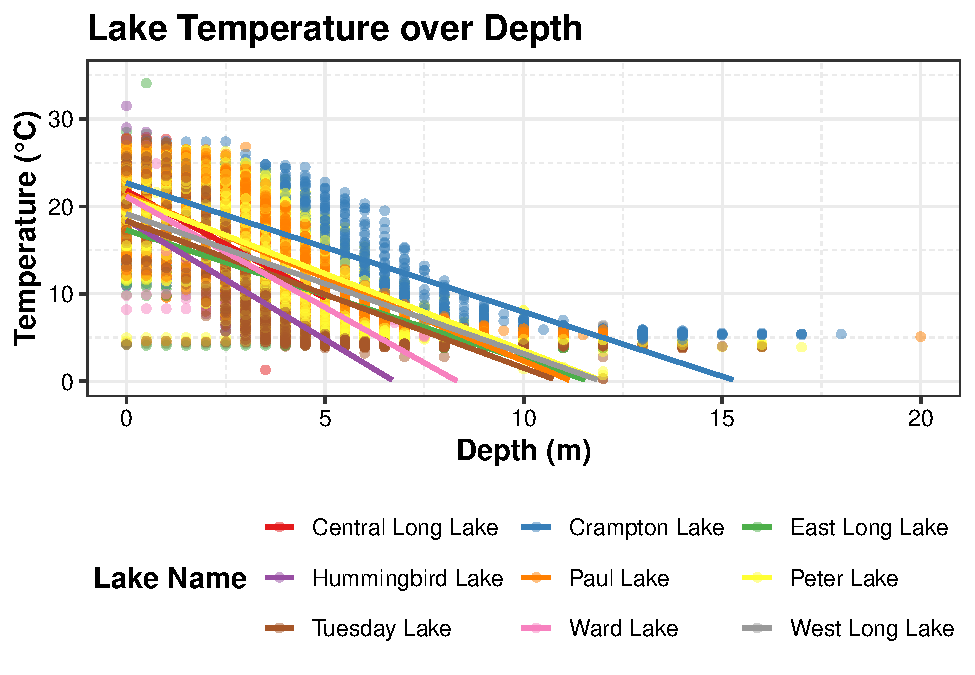
\includegraphics{A08_TimeSeries_files/figure-latex/unnamed-chunk-6-1.pdf}


\end{document}
